\subsection{RELIEF: Intelligent Repeaters and Robots for Fast, Reliable, Low-Cost RFID Inventorying \& Localization}

Context: Project co-financed by EU and Greek National Funds, under the call RESEARCH - CREATE -INNOVATE (project code: T1EDK-03032); Aristotle University of Thessaloniki, Greece\\

\noindent Duration: 09/2018--09/2021\\

\noindent \href{http://relief.web.auth.gr/language/en/home/}{\texttt{[Website]}} \href{https://www.facebook.com/ReliefAuth}{\texttt{[fb]}} \href{https://www.youtube.com/@antonidimi/search?query=relief}{\texttt{[Videos]}} \href{https://relief.web.auth.gr/language/en/publications/}{\texttt{[Publications]}} \\

Inventorying and localisation of products in large warehouses is constrained by
the accuracy and stamina of focus of human-led efforts. If RFID tags substitute
(optical!) bar codes, both needs may be fulfilled with greater accuracy and in
less time. If, additionally, robots replace humans, their time may be liberated
for other, more engaging/demanding activities, and errors may be erased.

The aim of project RELIEF was to provide Real-time Simultaneous Robot
Localisation and Mapping of RFID tags in 3D space with centimeter accuracy. The
means of achieving these goals were Unmanned
\href{https://www.youtube.com/watch?v=bo4lMI640DY}{Ground} and
\href{https://www.youtube.com/watch?v=9YpBIaO4tgY}{Aerial} Vehicles.

\begin{figure}[H]\centering
  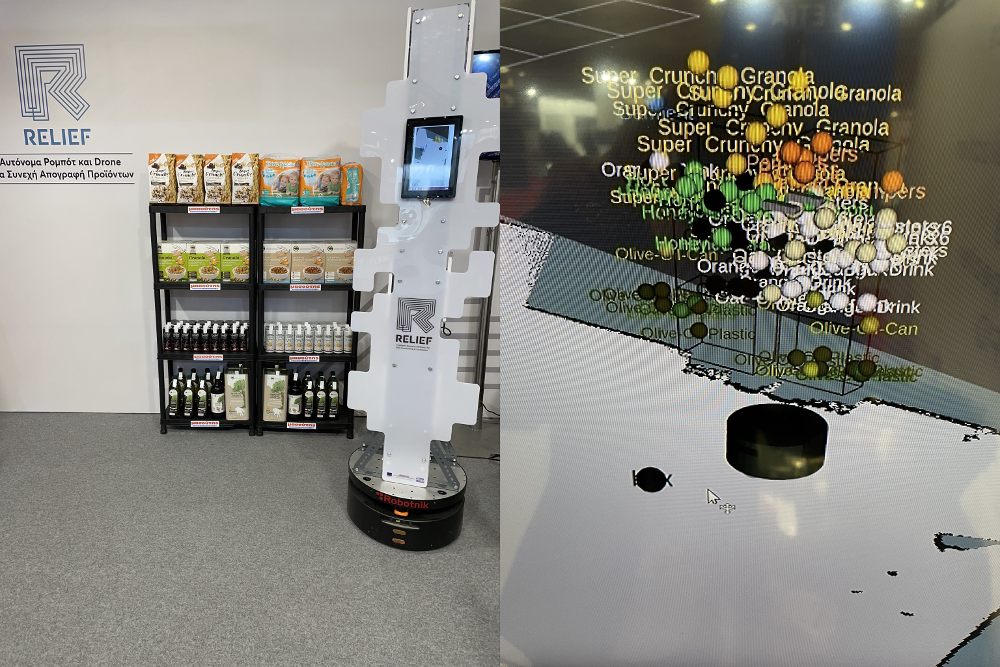
\includegraphics[scale=0.4]{images/relief_1.png}
  \caption{}
  \label{fig:relief_1}
\end{figure}

\begin{figure}[H]\centering
  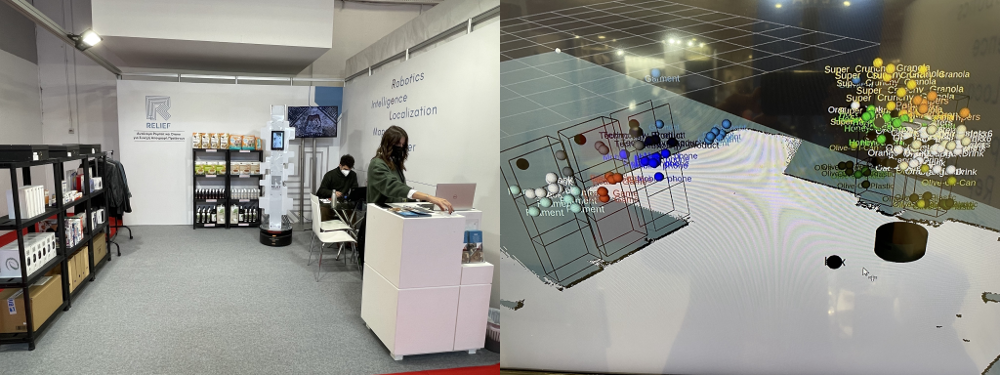
\includegraphics[scale=0.4]{images/relief_2.png}
  \caption{}
  \label{fig:relief_2}
\end{figure}


\begin{itemize}
\item Notions/resources/tools used: ROS, Linux, Hokuyo LIDAR, SLAM, Depth ASTRA Cameras, \texttt{amcl}, git, \texttt{RTAB-Map}, Impinj R420 RFID Reader
\item Publications resulted from this work: \cite{8739423,8739486,Filotheou2020a,9109328,9244904,Filotheou2020b,9566425,9617436}
\end{itemize}
